\documentclass[tikz,margin=0.6mm]{standalone}

% pdftk jigsaw.pdf burst  output jigsaw%02d.pdf
% pdftocairo -singlefile -transp -r 250 -png jigsaw01.pdf jigsaw01

\usepackage{amsmath}
\usepackage{amssymb}
\usepackage{physics} % \usepackage[arrowdel]{physics}
\usepackage{txfonts} % times for math (for consistency)
\usepackage{times}
\usepackage{jigsaw}

\usetikzlibrary{calc}

\gdef\sigb{\vb*{\sigma}}
\gdef\taub{\vb*{\tau}}
\gdef\epsb{\dot{\vb*{\epsilon}}}
\gdef\eps#1{\dot{\epsilon}_{#1}}
\gdef\statevec{\vb{s}}
\gdef\bulkvisc{\vb*{\eta}}
\gdef\bulkvisc{E_{ij}}

%\gdef\mygray{black!9!white}
\definecolor{mydarkgray}{RGB}{200,200,200} 
\definecolor{mygray}{RGB}{240,240,240} 

\definecolor{colorFL}{RGB}{198,219,239} % flow law 
\definecolor{colorMB}{RGB}{218,218,235} % momentum balance
\definecolor{colorFM}{RGB}{199,233,192} % fabric model
\definecolor{colorVA}{RGB}{253,208,162} % viscous anisotropy

\gdef\asp{0.75}
\gdef\asp{0.85}
\gdef\scale{2.0}

\gdef\mylarge#1{ #1 }
\gdef\mysmall#1{ {\fontsize{6.0}{6.0}\selectfont #1} }

\tikzset{every picture/.style={line cap=rect,line width=0.6pt}}

\newcommand{\blockFL}[1]{
	\begin{scope}[xshift=0cm,yshift=1cm]
	    \color{black}
	    \piece[#1]{1}{-1}{0}{0}
	    \color{black}    
	    \node at (0.5,0.55) {\mylarge{$\taub(\epsb,\bulkvisc, \vb{m}_i, \cdots)$}};
	    \node[anchor=west] (FL) at ({(0)},{(0.9)}) {\mysmall{Bulk rheology}};
	\end{scope}   
}

\newcommand{\blockMB}[1]{
\begin{scope}[xshift=1cm,yshift=1cm]
    \color{black}
    \piece[#1]{-1}{0}{0}{1}
    \color{black}    
    \node at (0.630,0.53) {\mylarge{$-\div\sigb=\rho\vb{g}$}};
    \node at (0.630,0.37) {\mylarge{$\sigb=\taub-p\vb{I}$}};
    \node[anchor=east] (MB) at ({(1)},{(0.9)}) {\mysmall{Momentum balance}};
\end{scope}   
}

\newcommand{\blockFM}[1]{
\begin{scope}[xshift=1cm,yshift=0cm]
    \color{black}
    \piece[#1]{0}{0}{1}{-1}
    \color{black}
	\node at ({0.5},0.45) {\mylarge{$\dfrac{\mathrm{D} \statevec}{\mathrm{D} t} = \vb{M}\statevec$}};
    \node[anchor=east] (FM) at ({1},0.1) {\mysmall{Fabric evolution}};
\end{scope}    
}

\newcommand{\blockVA}[1]{
\begin{scope}[xshift=0cm,yshift=0cm]
    \color{black}
    \piece[#1]{0}{1}{-1}{0}
    \color{black}
	\node[align=left] at ({0.38},0.47) {\mylarge{$\bulkvisc(\statevec)$, $\vb{m}_i(\statevec)$}};
	\node[anchor=west,align=left] (VA) at ({0},0.10) {\mysmall{Viscous anisotropy}};
\end{scope}   
}

\usepackage{pgfplots}
\usetikzlibrary{patterns}
\usetikzlibrary{shapes}
\usetikzlibrary{backgrounds}
\usetikzlibrary{decorations.pathmorphing}
\usetikzlibrary{decorations.markings}
\usetikzlibrary{shadows} 

\definecolor{bgcolor}{HTML}{f7f6ee} % grayish

\tikzset{
	projboxtitle/.style={darkgray, line width=0.6pt, align=left, draw=darkgray, inner sep=1.5ex, font=\fontsize{5pt}{5pt}\selectfont, fill=bgcolor!50, }, % drop shadow={shadow xshift=0.6ex,shadow yshift=-0.6ex},
	projbox/.style={line cap=butt, align=left, yshift=-0.4em, xshift=1em,	darkgray, line width=2pt, font=\fontsize{9pt}{9pt}\selectfont, rectangle, },
}

\begin{document}

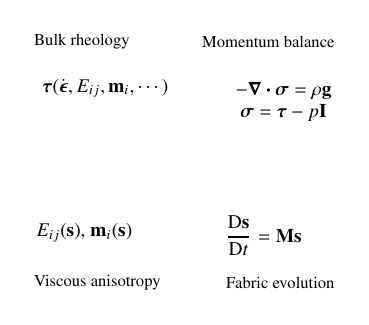
\begin{tikzpicture}[xscale=\scale,yscale={\scale*\asp}]
\scriptsize
\blockFL{colorFL}
\blockMB{colorMB}
\blockVA{colorVA}
\blockFM{colorFM}
\end{tikzpicture}

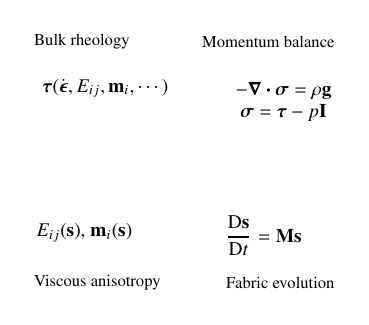
\begin{tikzpicture}[xscale=\scale,yscale={\scale*\asp}]
\scriptsize
\blockFL{mygray}
\blockMB{mygray}
\blockVA{mygray}
\blockFM{colorFM}
\end{tikzpicture}

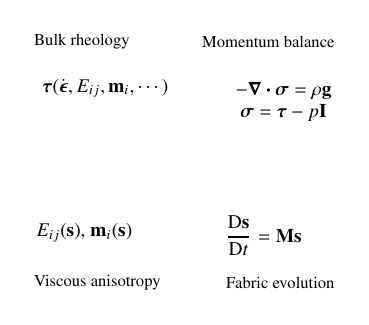
\begin{tikzpicture}[xscale=\scale,yscale={\scale*\asp}]
\scriptsize
\blockFL{mygray}
\blockMB{mygray}
\blockVA{colorVA}
\blockFM{mygray}
\end{tikzpicture}

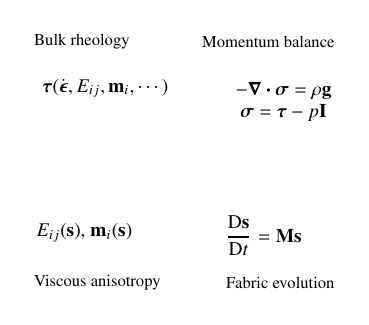
\begin{tikzpicture}[xscale=\scale,yscale={\scale*\asp}]
\scriptsize
\blockFL{colorFL}
\blockMB{mygray}
\blockVA{mygray}
\blockFM{mygray}
\end{tikzpicture}

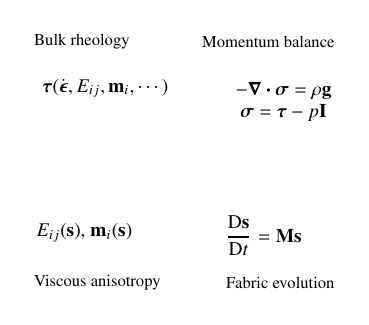
\begin{tikzpicture}[xscale=\scale,yscale={\scale*\asp}]
\scriptsize
\blockFL{mygray}
\blockMB{colorMB}
\blockVA{mygray}
\blockFM{mygray}
\end{tikzpicture}


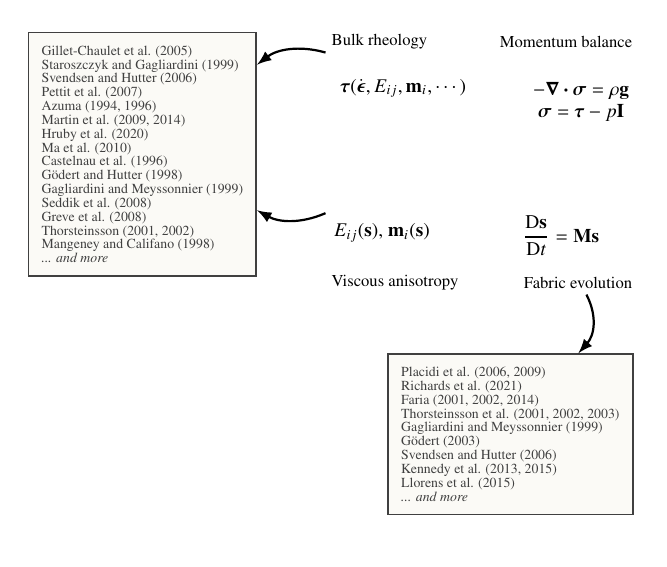
\begin{tikzpicture}[xscale=\scale,yscale={\scale*\asp}]
	
	\scriptsize
	\blockFL{colorFL}
	\blockMB{colorMB}
	\blockVA{colorVA}
	\blockFM{colorFM}

	\gdef\litbox#1#2#3#4#5{
		\node[projboxtitle] (#5) at (#1,#2) {#3};
		\node[] (#5box) [projbox, anchor=north west] at (#5.south west) {#4};
	}
	
	\litbox{4.8em}{-4.2em}{Placidi et al. (2006, 2009)\\ Richards et al. (2021)\\ Faria (2001, 2002, 2014) \\ Thorsteinsson et al. (2001, 2002, 2003) \\ Gagliardini and Meyssonnier (1999) \\ Gödert (2003) \\ Svendsen and Hutter (2006) \\ Kennedy et al. (2013, 2015) \\ Llorens et al. (2015) \\ \textit{... and more}}{}{FMbox}
	
	\litbox{-4.7em}{4.3em}{Gillet-Chaulet et al. (2005)\\ Staroszczyk and Gagliardini (1999) \\ Svendsen and Hutter (2006) \\ Pettit et al. (2007) \\ Azuma (1994, 1996)\\ Martin et al. (2009, 2014) \\ Hruby et al. (2020) \\ Ma et al. (2010) \\ Castelnau et al. (1996)\\ Gödert and Hutter (1998)\\ Gagliardini and Meyssonnier (1999)\\ Seddik et al. (2008) \\ Greve et al. (2008) \\ Thorsteinsson (2001, 2002) \\ Mangeney and Califano (1998) \\ \textit{... and more}}{}{FLbox}
	
	\gdef\arrlen{2em}
	\draw[-latex, thick] (FM) to[bend left] (FMbox.50);
	\draw[-latex, thick] (0,7.4em) to[bend right] (FLbox.38);
	\draw[-latex, thick] (0,2.5em) to[bend left] (FLbox.334);

\end{tikzpicture}

\end{document}
